\section{Charts}

\begin{figure}[!htb]
	\centering
	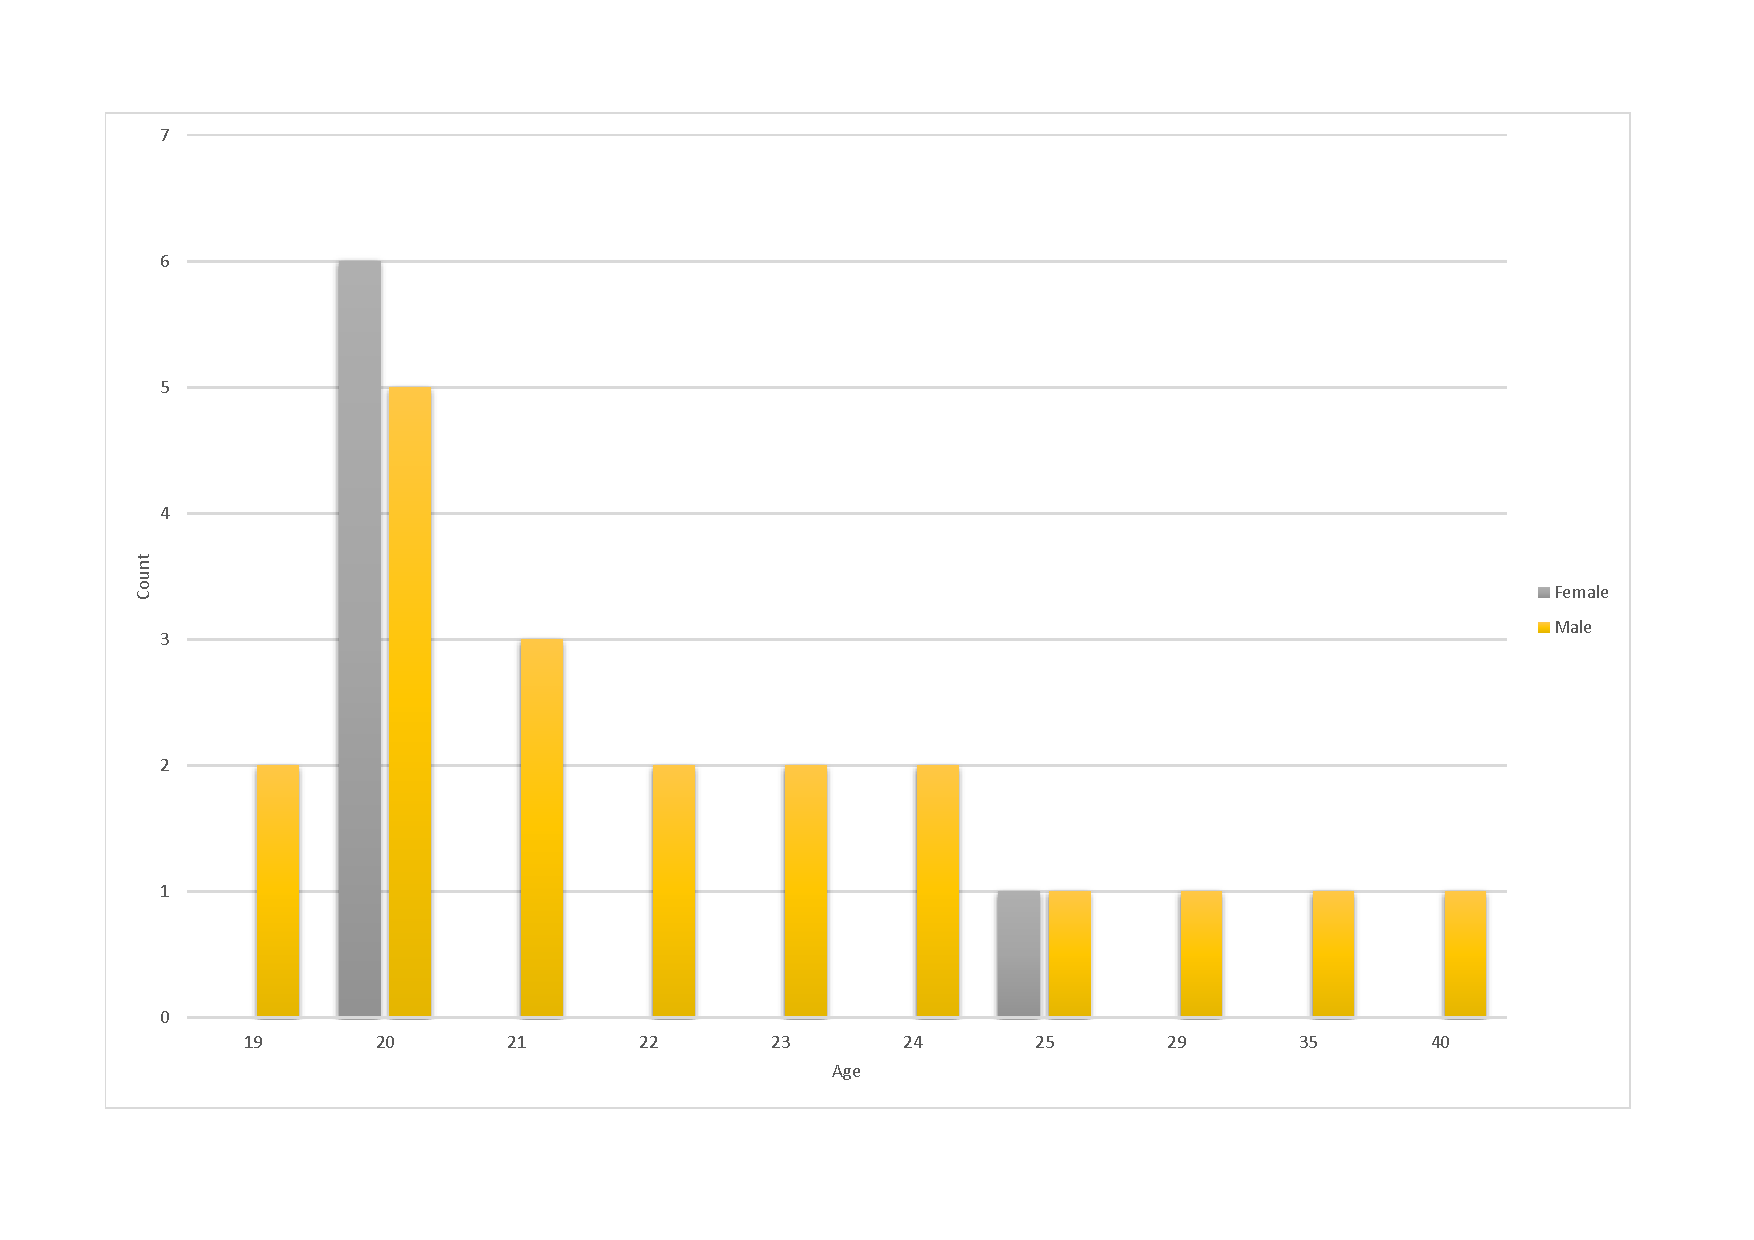
\includegraphics[height=7cm]{charts/genderAge.pdf}
	\caption[Sample age and gender]{Count Participants' gender and age }
	\label{fig:chart-genderage}
\end{figure}

\begin{figure}[!htb]
	\centering
	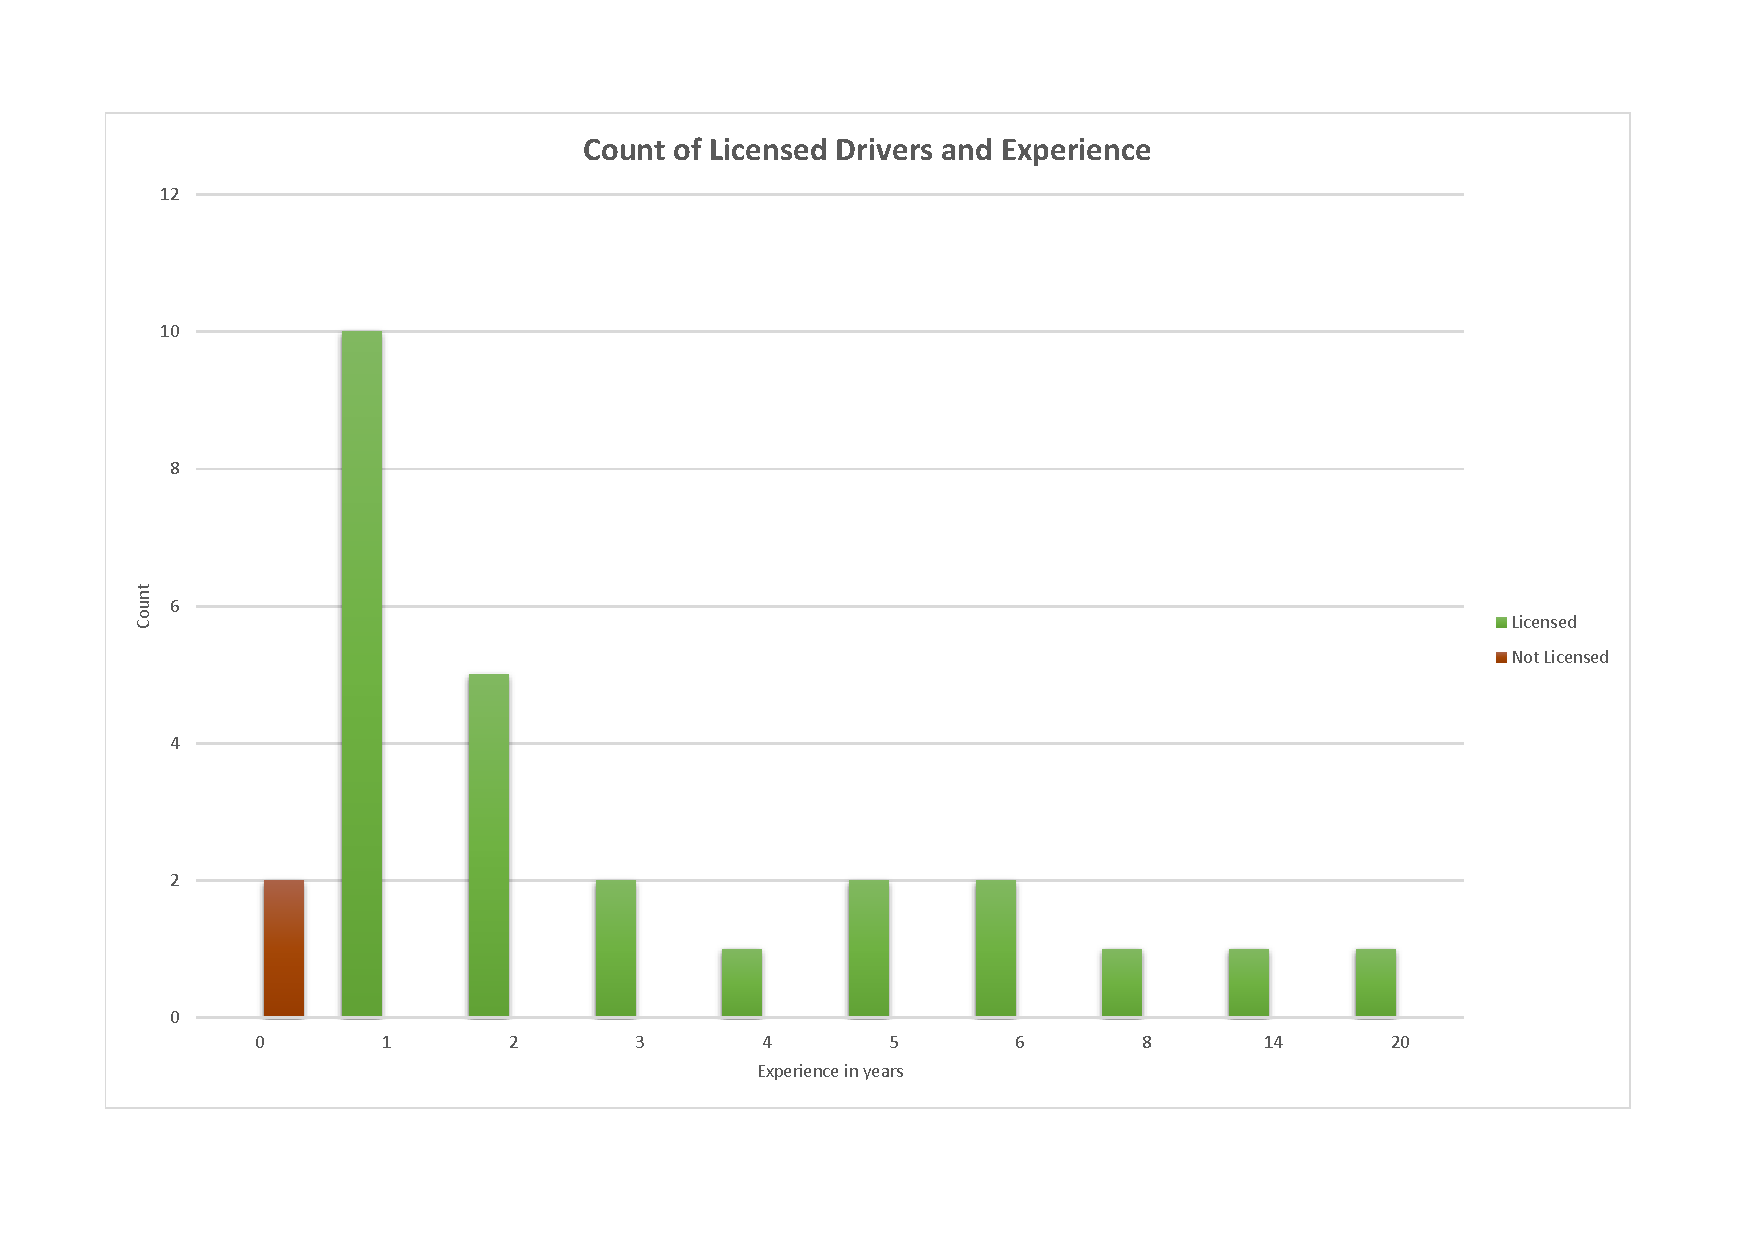
\includegraphics[height=7cm]{charts/licenseddriversexperience.pdf}
	\caption[Licensed drivers experience]{Licensed drivers and experience}
	\label{fig:chart-licenseddriversexperience}
\end{figure}

\begin{figure}[!htb]
	\centering
	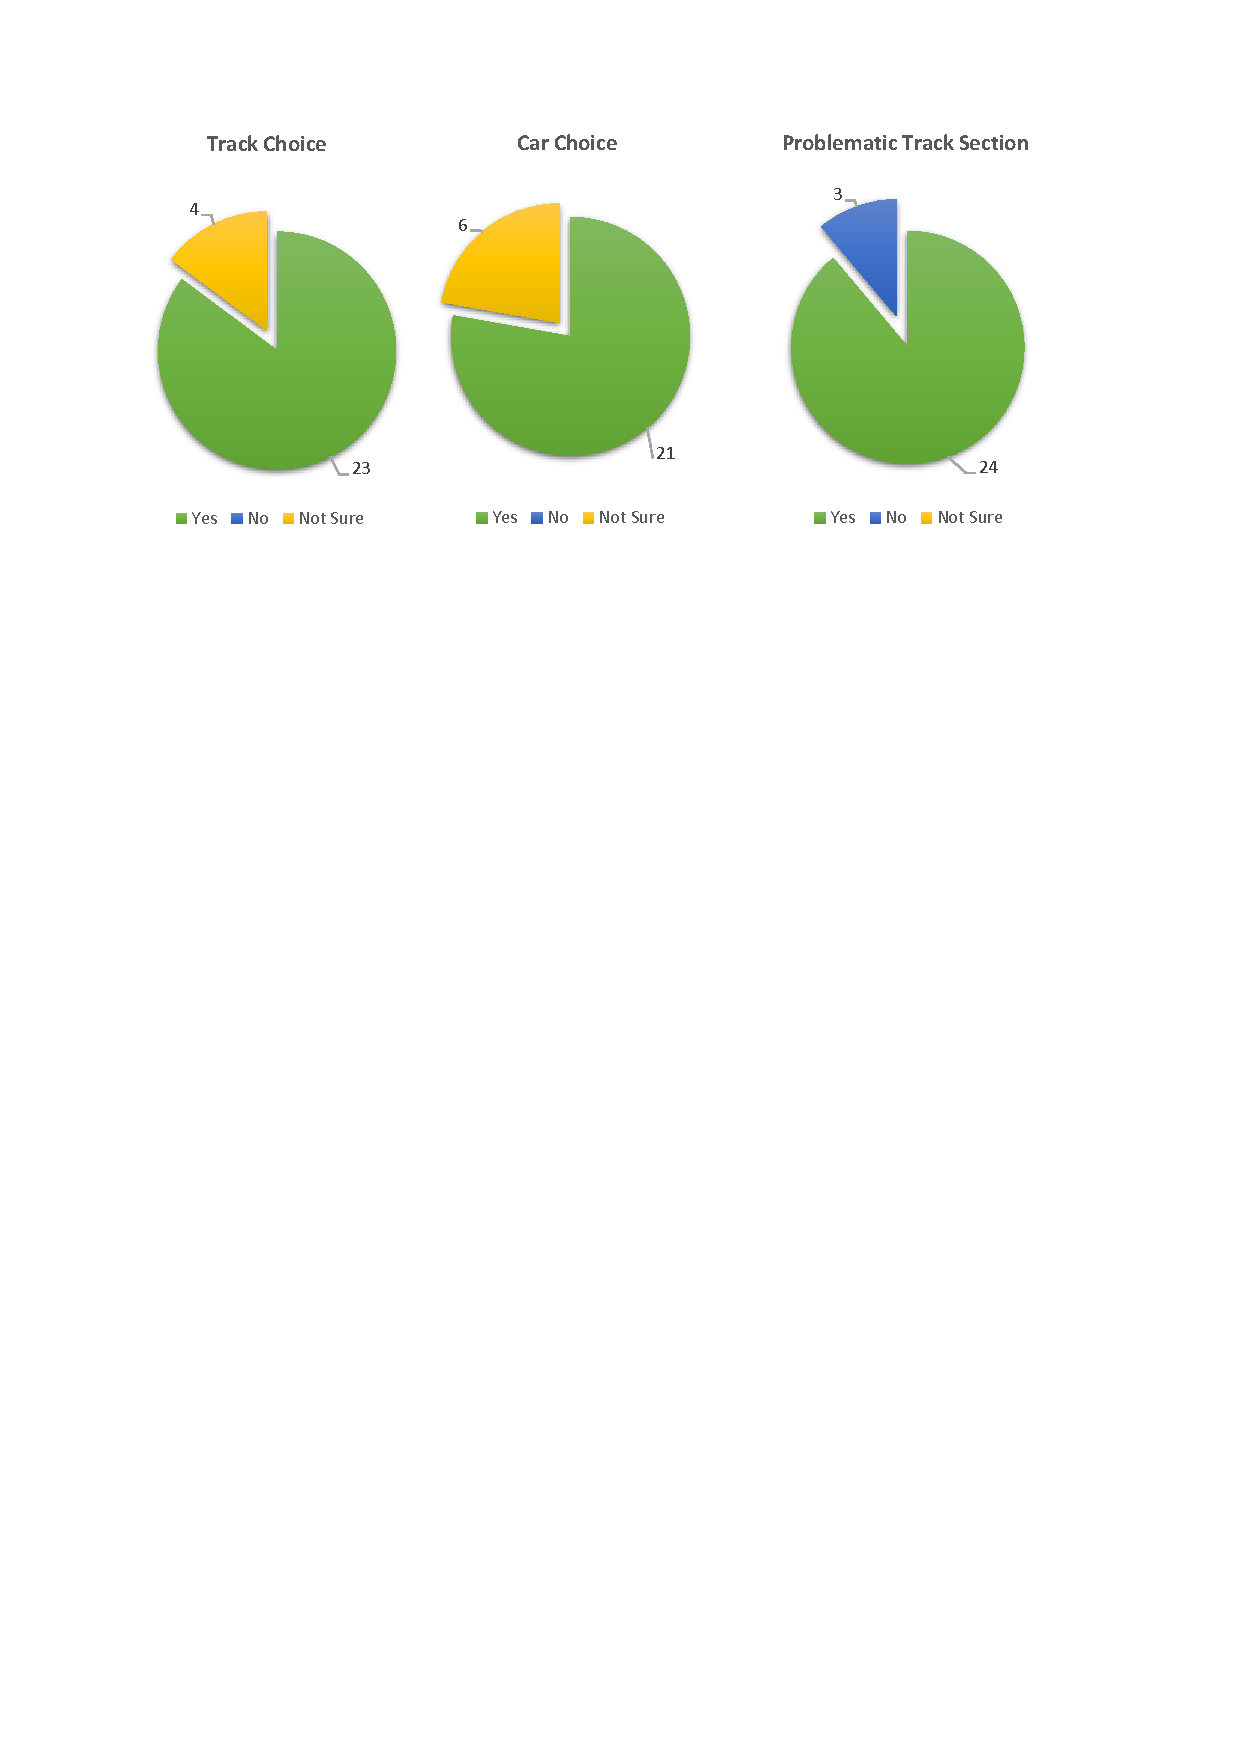
\includegraphics[height=5cm]{charts/choices.pdf}
	\caption{Where the track and car choice adequet?}
	\label{fig:chart-choices}
\end{figure}

\begin{figure}[!htb]
	\centering
	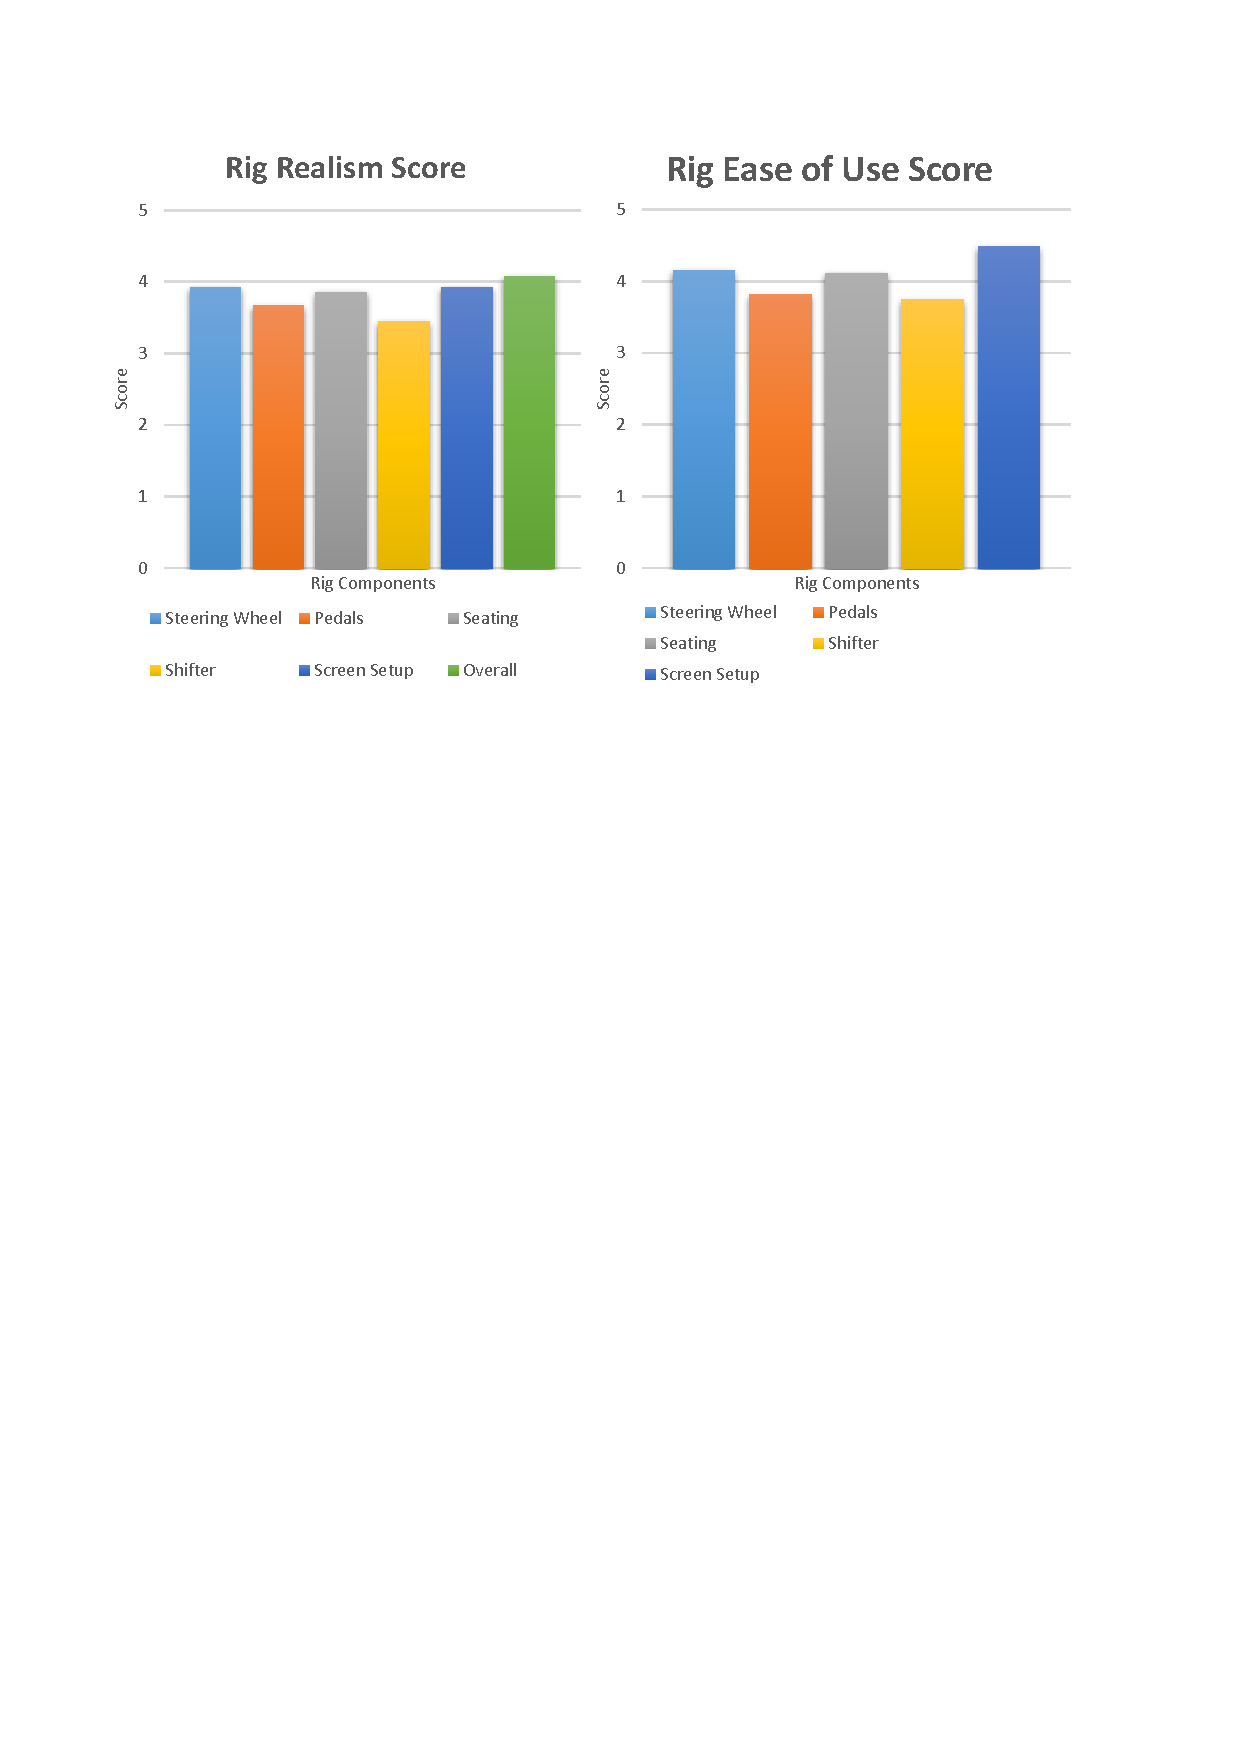
\includegraphics[height=7cm]{charts/realistic.pdf}
	\caption{How real do these componets feel?}
\label{fig:chart-realistic}
\end{figure}

\begin{figure}[!htb]
	\centering
	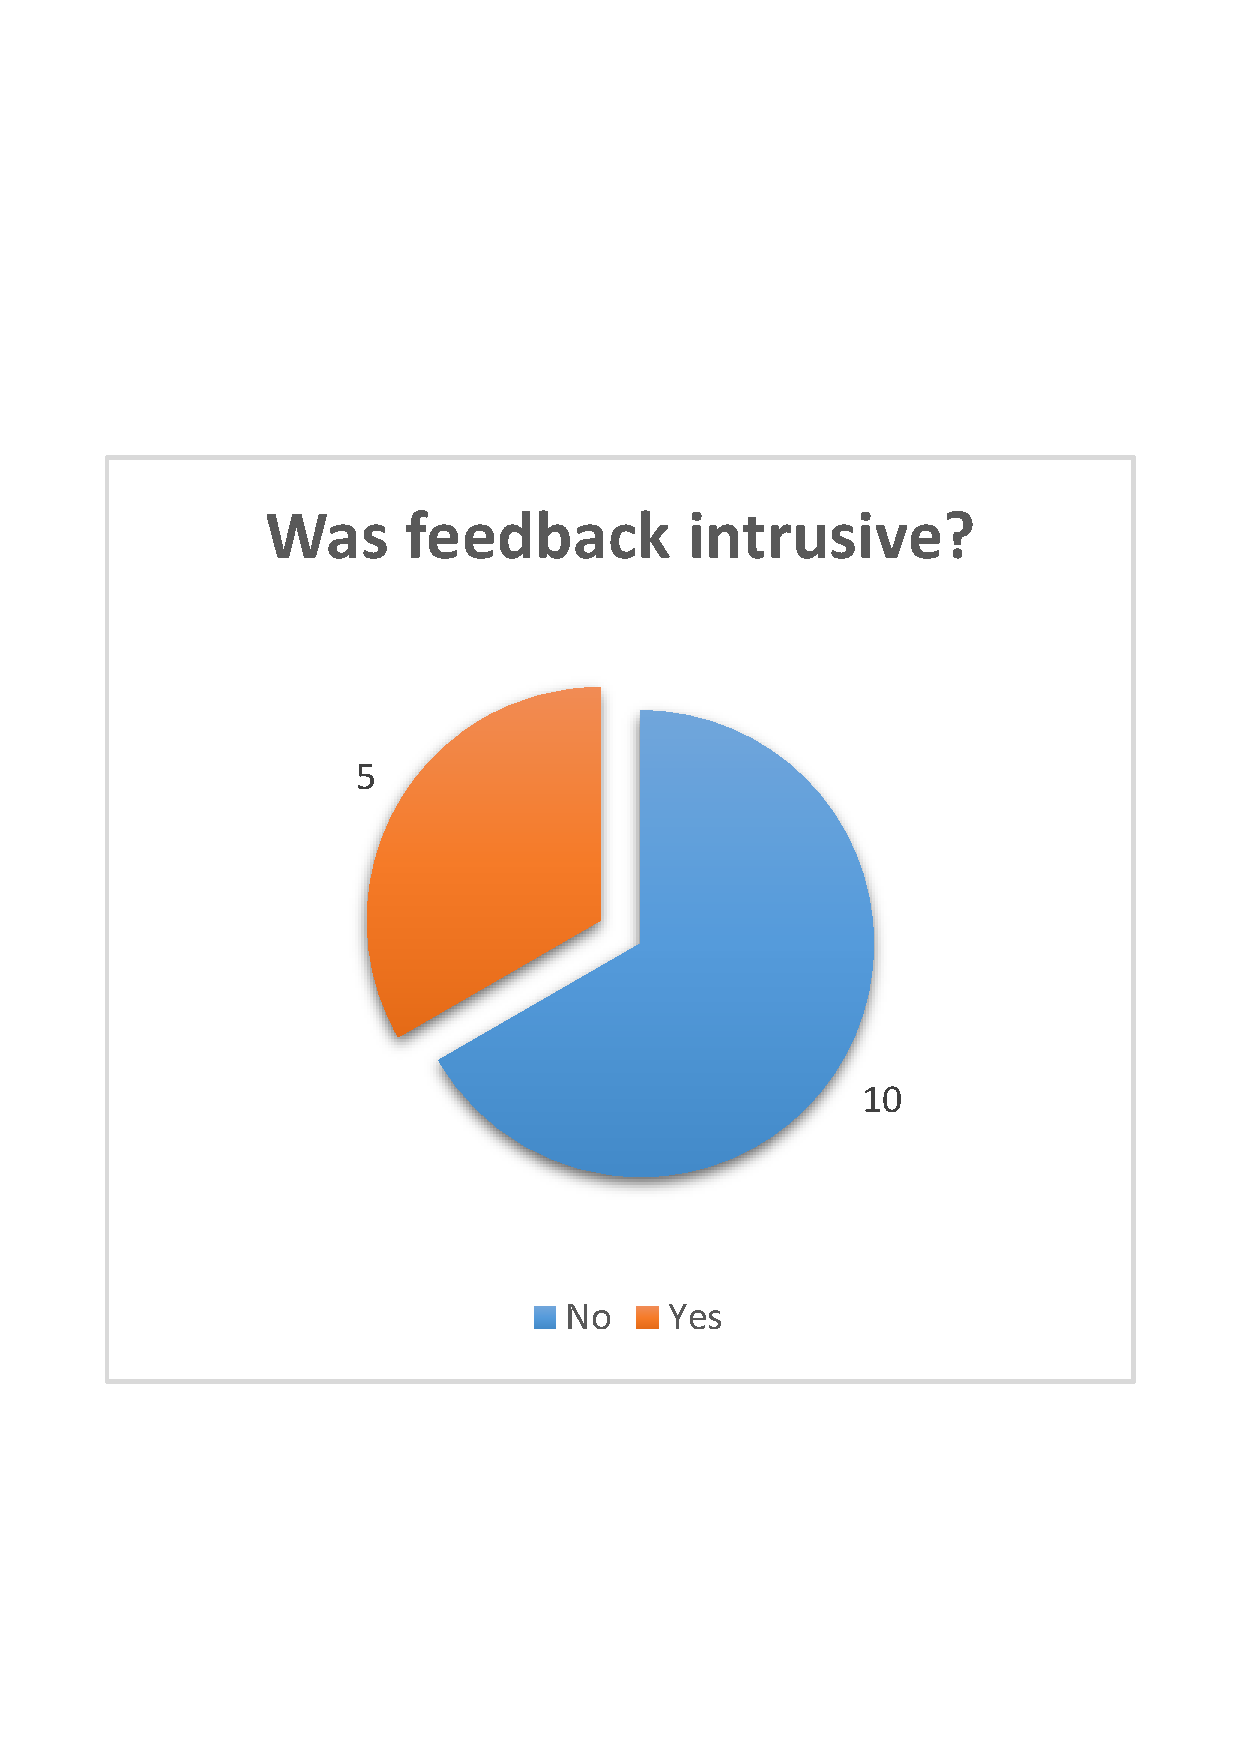
\includegraphics[height=7cm]{charts/intrusivefeedback.pdf}
	\caption{Was the feedback intrusive?}
\label{fig:chart-intrusivefeedback}
\end{figure}

Transcript of the audio files